\model{Version Control Scenarios}
  \begin{center}
    \small
    \begin{tabular}{p{1.25in}p{1.75in}p{2.25in}}
      \begin{minipage}{1.25in}
        \centering
        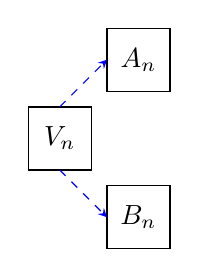
\begin{tikzpicture}[scale=0.8]
          \draw (0,0) rectangle (1,1);
          \node at (0.5,0.5) {$V_n$};
          \draw (1.25,1.25) rectangle (2.25,2.25);
          \node at (1.75,1.75) {$A_n$};
          \draw (1.25,-0.25) rectangle (2.25,-1.25);
          \node at (1.75,-0.75) {$B_n$};
          \draw[blue,dashed,-stealth] (0.5,1) -- (1.25,1.75);
          \draw[blue,dashed,-stealth] (0.5,0) -- (1.25,-0.75);
        \end{tikzpicture}\par
        Scenario \#1
      \end{minipage}
      &
      \begin{minipage}{1.75in}
        \centering
        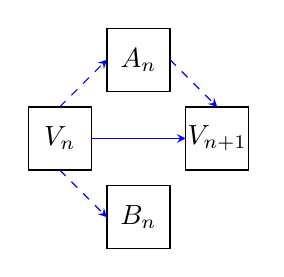
\begin{tikzpicture}[scale=0.8]
          \draw (0,0) rectangle (1,1);
          \node at (0.5,0.5) {$V_n$};
          \draw (1.25,1.25) rectangle (2.25,2.25);
          \node at (1.75,1.75) {$A_n$};
          \draw (1.25,-0.25) rectangle (2.25,-1.25);
          \node at (1.75,-0.75) {$B_n$};
          \draw (2.5,0) rectangle (3.5,1);
          \node at (3,0.5) {$V_{n+1}$};
          \draw[blue,dashed,-stealth] (0.5,1) -- (1.25,1.75);
          \draw[blue,dashed,-stealth] (0.5,0) -- (1.25,-0.75);
          \draw[blue,dashed,-stealth] (2.25,1.75) -- (3,1);
          \draw[blue,-stealth] (1,0.5) -- (2.5,0.5);
        \end{tikzpicture}\par
        Scenario \#2
      \end{minipage}
      &
      \begin{minipage}{2.25in}
        \centering
        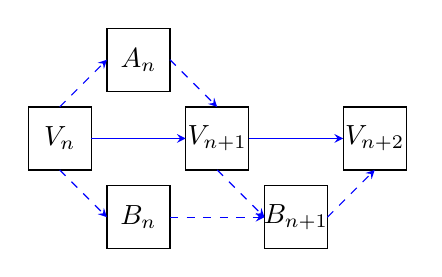
\begin{tikzpicture}[scale=0.8]
          \draw (0,0) rectangle (1,1);
          \node at (0.5,0.5) {$V_n$};
          \draw (1.25,1.25) rectangle (2.25,2.25);
          \node at (1.75,1.75) {$A_n$};
          \draw (1.25,-0.25) rectangle (2.25,-1.25);
          \node at (1.75,-0.75) {$B_n$};
          \draw (2.5,0) rectangle (3.5,1);
          \node at (3,0.5) {$V_{n+1}$};
          \draw (3.75,-0.25) rectangle (4.75,-1.25);
          \node at (4.25,-0.75) {$B_{n+1}$};
          \draw (5,0) rectangle (6,1);
          \node at (5.5,0.5) {$V_{n+2}$};
          \draw[blue,dashed,-stealth] (0.5,1) -- (1.25,1.75);
          \draw[blue,dashed,-stealth] (0.5,0) -- (1.25,-0.75);
          \draw[blue,dashed,-stealth] (2.25,1.75) -- (3,1);
          \draw[blue,-stealth] (1,0.5) -- (2.5,0.5);
          \draw[blue,dashed,-stealth] (2.25,-0.75) -- (3.75,-0.75);
          \draw[blue,dashed,-stealth] (3,0) -- (3.75,-0.75);
          \draw[blue,dashed,-stealth] (4.75,-0.75) -- (5.5,0);
          \draw[blue,-stealth] (3.5,0.5) -- (5,0.5);
        \end{tikzpicture}\par
        Scenario \#3
      \end{minipage}
    \end{tabular}
  \end{center}

  {\it\large Refer to Model 1 above as your team develops consensus answers
    to the questions below.}

  \quest{25 min}
    
  \Q A {\it version control system} (VCS) helps to manage
    multiple versions of files, such as program source code.  Such a
    collection of files is called a {\it repository}.  In the
    model above, $V_n$ represents the current version of the
    repository. If Amy and Bob are two developers working on the code
    stored in $V_n$, they will first {\it check out} their own local copies,
    $A_n$ and $B_n$, of the repository to edit. The first scenario of
    the model depicts this situation.
    \par\vskip 10pt
    \begin{enumerate}
      \item What do the dashed arrows represent?
        \begin{answer}[0.75in]
          The dashed lines represent a checkout or copy of the repository
          to edit in a local environment.
        \end{answer}

      \item Why is it better for Amy and Bob to edit their own copies
        of the repository rather than files in $V_n$ directly?
        \begin{answer}[1in]
          As developers make changes the code will likely be broken, so 
          it is better for changes not to be visible to others till the
          development and testing process is done.
        \end{answer}

      \item What problems might result from Amy and Bob editing
        their own copies of the repository?
        \begin{answer}[0.75in]
          They will not get changes (fixes and features) added by others, 
          so the changes they make will not be compatible with the current
          version in the repository.
        \end{answer}
    \end{enumerate}

  \newpage
    
  \Q After editing, Amy adds her changes to the main repository
    to create a new version, $V_{n+1}$.  We say that Amy
    {\it commits} changes to the repository.  This is shown in
    the second scenario.
    \begin{enumerate}
      \item How is Amy's commit shown in the diagram for scenario \#2?
        \begin{answer}[0.75in]
          There are dashed lines from Amy's copy to the new version and
          a solid line from the previous version to the new version.
        \end{answer}

      \item Before Amy commits her code, can Bob view Amy's changes?
        Explain.
        \begin{answer}[0.75in]
          Amy's edits are in Amy's environment, not in the shared 
          repository. So, no, Bob cannot view Amy's changes (unless he 
          has access to Amy's environment through other means).
        \end{answer}

      \item Why is it important that Amy test her code before she
        commits it?
        \begin{answer}[0.75in]
          Once Amy commits her code to the shared repository, then other 
          developers will start using it. If it is broken then other 
          developers will be impacted.
        \end{answer}
    \end{enumerate}

  \vskip -20pt
    
  \Q Before Bob can commit his changes, he must get all of Amy's
    changes from $V_{n+1}$.  We say that Bob {\it updates} his local
    copy from the repository.  This is depicted in the third scenario.
    \begin{enumerate}
      \item Why must Bob update his local copy before he can commit
        changes to the repository?
        \begin{answer}[0.75in]
          Bob should make sure that he does not accidentally overwrite
          or replace Amy's changes. He should also make sure that his 
          changes are compatible with Amy's changes. It could be that 
          Amy's changes work in isolation, and Bob's changes work in 
          isolation, but together they do not work. 
        \end{answer}

      \item Why are there two arrows pointing to $B_{n+1}$, Bob's
        updated copy of the repository, instead of one?
        \begin{answer}[0.75in]
          Bob's new copy has changes from both sources.
        \end{answer}

      \item What should Bob do before he commits his updated changes
        back to the main repository?
        \begin{answer}[0.75in]
          Bob should review Amy's changes to see if they conflict with 
          his changes. Bob should also thoroughly test the merged code.
        \end{answer}
    \end{enumerate}
    
  \Q Which of the operations discussed in this model ({\it
    checkout}, {\it commit}, and {\it update}) are\key\\[-2.5mm] best described
    by the following?
    \begin{enumerate}
      \itemsep 10pt
      \item Transfers the most amount of data:
        \hfill \ans[2.5in]{checkout}

      \item Transfers the least amount of data:
        \hfill \ans[2.5in]{commit (an update may have several commits)}

      \item Might result in a {\it conflict} between file versions:
        \hfill \ans[2.5in]{[update (or a commit without an update)}
    \end{enumerate}
    
  \Q We can use {\it timeline diagrams} such as those shown in the
    model to visualize versions ({\it nodes} represented by
    rectangles) and connections ({\it links} represented by arrows). 
    Draw a timeline diagram to show the following sequence of events.
    \begin{center}
      \begin{minipage}{4.5in}
        \begin{enumerate}[i.]
          \itemsep -2pt
          \item We start with version 10 of the project files
          \item Amy checks out her own copy
          \item Amy edits and commits, creating a new version
          \item Bob checks out his own copy            
          \item Amy makes another edit and commits again
          \item Bob updates
          \item Bob edits and commits
        \end{enumerate}
      \end{minipage}
    \end{center}
    \par\vskip 15pt
    \begin{answer}[2in]
      Answers will vary
    \end{answer}